\documentclass{article}
\usepackage{float}
\usepackage{circuitikz}
\usepackage{cite}
\usepackage{amsmath,amssymb,amsfonts,amsthm}
\usepackage{algorithmic}
\usepackage{graphicx}
\usepackage{textcomp}
\usepackage{xcolor}
\usepackage{txfonts}
\usepackage{listings}
\usepackage{amsmath}
\usepackage{enumitem}
\usepackage{mathtools}
\usepackage{gensymb}
\usepackage{comment}
\usepackage[breaklinks=true]{hyperref}
\usepackage{tkz-euclide} 
\usepackage{listings}
\usepackage{gvv}        

%Enumering lower case roman numerals
%\renewcommand{\theenumi}{\roman{enumi}}   
%\renewcommand{\labelenumi}{\theenumi)}


\begin{document}

\title{ \textbf{Filter Design}}

\author{Kamale Goutham\\EE23BTECH11028}
\date{}

\maketitle
%-------------------------------------------------------------------------------
\section{Introduction}
We are supposed to design the equivalent FIR and IIR filter realizations for filter number.  
This is a bandpass filter whose specifications are available below.

\section{Filter Specifications}
The sampling rate for the filter has been specified as $F_s =  48$ kHz.	If the un-normalized  discrete-time (natural) frequency is F, the corresponding normalized digital filter (angular) frequency is given by $\omega = 2\pi
\left(\frac{F}{F_s}\right)$.

\subsection{The Digital Filter}

\begin{enumerate}
\item {\em Tolerances:}  The passband ($\delta_1$) and stopband ($\delta_2$) tolerances are given to
be equal, so we let $\delta_1 = \delta_2 = \delta = 0.15$.

\item {\em Passband:}  The passband is from \{4 + 0.6(j)\}kHz
to \{3 + 0.6(j+2)\}kHz.
where 
\begin{align}
    j=\brak{r-11000} \mod \sigma
\end{align}
where $\sigma$ is sum of digits of roll number and $r$ is roll number.\\
\begin{align}
    r&=11224\\
    \sigma  &= 10\\
    j&=4
\end{align}
substituting $j = 114$ gives the passband range for our bandpass filter as $6.4$ kHz - $7.6$ kHz.  Hence, the un-normalized discrete time filter
passband frequencies are $F_{p1} = 7.6$ kHz
and $F_{p2} = 6.4$ kHz.  The corresponding normalized digital filter passband frequencies are
$\omega_{p1} = 2\pi\frac{F_{p1}}{F_s}  = 0.317\pi$  and $\omega_{p2} = 2\pi\frac{F_{p2}}{F_s}  = 0.267 \pi$ kHz.  The centre frequency is then given by  $\omega_c = \frac{\omega_{p1} + \omega_{p2}}{2} = 0.292\pi$.  

\item {\em Stopband:}  The {\em transition band} for bandpass filters is $\Delta F = 0.3$ kHz on either side of the passband.
Hence, the un-normalized {\em stopband} frequencies are $F_{s1} = 7.6 + 0.3 = 7.9$ kHz and $F	_{s2} = 6.4 - 0.3 = 6.1$ kHz.  The corresponding normalized frequencies are $\omega_{s1} = 0.329 \pi$  and $\omega_{s2} =  0.254 \pi$.
\end{enumerate}

\subsection{The Analog filter}
In the bilinear transform, the analog filter frequency ($\Omega$) is related to the corresponding digital filter frequency ($\omega$) as $\Omega = \tan \frac{\omega}{2}$.  Using this relation, we obtain the analog passband and stopband frequencies as $\Omega_{p1} = 0.5429$, $\Omega_{p2} = 0.4452$ and $\Omega_{s1} = 0.5687$, $\Omega_{s2} = 0.4219$
respectively.

\section{The IIR Filter Design}
{\em Filter Type:}  We are supposed to design filters whose stopband is monotonic and passband equiripple.  
Hence, we use the {\em Chebyschev approximation} to design our bandpass IIR filter.

\subsection{The Analog Filter}
\begin{enumerate}
\item {Low Pass Filter Specifications:}  Let $H_{a, BP}(j\Omega)$ be the desired analog bandpass filter,  with the specifications provided in Section 2.2, and $H_{a,LP}(j\Omega_L)$ be the equivalent low pass filter, then
\begin{equation}
\Omega_L = \frac{\Omega^2 - \Omega_0^2}{B\Omega} \label{eq:freq_transform}
\end{equation}
where $\Omega_0 = \sqrt{\Omega_{p1}\Omega_{p2}} = 0.49167$ and $B = \Omega_{p1} - \Omega_{p2} = 0.0977$.

Substituting $\Omega_{s1}$ and $\Omega_{s2}$ in \eqref{eq:freq_transform} we obtain the stopband edges of lowpass filter 
\begin{align}
    \Omega_{Ls1} &= \frac{\Omega_{s1}^2 - \Omega_0^2}{B\Omega_{s1}} = 1.4689\\
    \Omega_{Ls2} &= \frac{\Omega_{s2}^2 - \Omega_0^2}{B\Omega_{s2}} = -1.5459
\end{align}
And we choose the minimum of these two stopband edges
\begin{align}
    \Omega_{Ls} = \mbox{min}(\vert \Omega_{Ls_1}\vert,\vert \Omega_{Ls_2}\vert) = 1.4689.
\end{align}
\item {The Low Pass Chebyschev Filter Paramters:} The magnitude of frequency response of the low pass filter is given by 
\begin{align}
    \vert H_{a,LP}(j\Omega_L)\vert^2 = \frac{1}{1 + \epsilon^2c_N^2(\Omega_L/\Omega_{Lp})} \label{eq:mag_freq_response}
\end{align}
The passband edge of the low pass filter is chosen as $\Omega_{Lp}=1$.
Therfore ,
\begin{align}
    \vert H_{a,LP}(j\Omega_L)\vert^2 = \frac{1}{1 + \epsilon^2c_N^2(\Omega_L)} \label{eq:specification}
\end{align}
Here $c_N$ denote the chebyshev polynomials for a particular order $N$ of the filter.
\begin{align}
    c_N(x) &= \cosh(N \cosh^{-1}x) , x=\Omega_{L}\\
    c_0(x) &= 1 \\
    c_1(x) &= x
\end{align}
There exists a recurssive relation from which all the polynomials can be found out.
\begin{align}
    c_{N+2} &= 2xc_{N+1} - c_{N}  \label{eq:cheby_poly_relation}
\end{align}
Imposing the band restrictions on \eqref{eq:mag_freq_response} \\
\begin{align}
    \vert H_{a,LP}(j\Omega_L)\vert^2 < \delta_{2} \hspace{5pt} \text{for}\hspace{5pt} \Omega_L = \Omega_{Ls}\\
    1-\delta_{1}<\vert H_{a,LP}(j\Omega_L)\vert^2 < 1 \hspace{5pt} \text{for}\hspace{5pt} \Omega_L = \Omega_{Lp}\\
\end{align}
we obtain :
\begin{eqnarray}
\label{lpdesign}
\frac{\sqrt{D_2}}{c_N(\Omega_{Ls})} \leq \epsilon \leq \sqrt{D_1}, \nonumber \\
N \geq \left\lceil \frac{\cosh^{-1}\sqrt{D_2/D_1}}{\cosh^{-1}\Omega_{Ls}} \right\rceil,
\end{eqnarray}
where $D_1 = \frac{1}{(1 - \delta)^2}-1$ and $D_2 = \frac{1}{\delta^2} - 1$ and $\left \lceil . \right \rceil$ is known as the ceiling operator . 
\begin{table}[H]
    \centering
    
    \resizebox{0.49\textwidth}{!}{\begin{tabular}{|c|c|} % Define two centered columns with vertical lines
    \hline
    Parameter  & Value \\ % Row 1
    \hline
    $D_1$ & 0.384 \\ % Row 2
    \hline
    $D_2$ & 43.44 \\ % Row 3
    \hline
    $N$ & 4 \\ % Row 4
    \hline
    $c_4\brak{x}$ & $8x^4 + 8x^2 + 1$\\
    \hline
    \end{tabular}}
    \caption{Parameter Table} % Table caption
    \label{tab:par_tab} % Table label for reference
    \end{table}
we get $N\geq 4$ and $0.3141 \leq \epsilon \leq 0.61$\\
\newpage
The below code plots \eqref{eq:mag_freq_response} for different values of $\epsilon$ .
\begin{lstlisting}
https://github.com/yskp123/EE1205/tree/main/Filter_Design/codes/plot1.py
\end{lstlisting}
\begin{figure}[H]
\centering
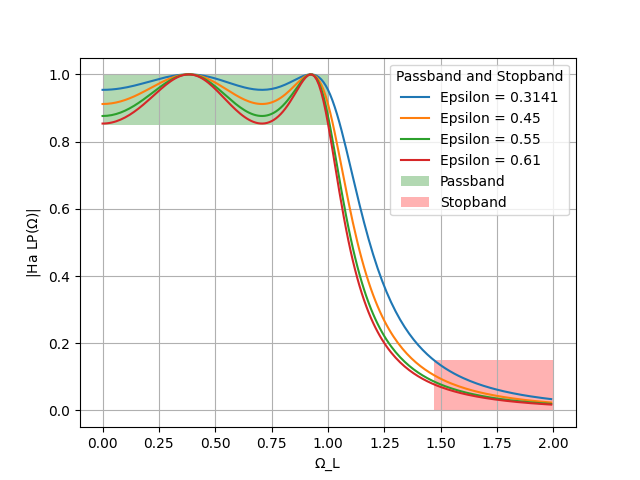
\includegraphics[width=1\columnwidth]{figs/plot1.png}
\caption{The Analog Low-Pass Frequency Response for $0.3141  \leq \epsilon \leq 0.61$}
\label{fig:H_for_diff_eb}
\end{figure}

In \figref{fig:H_for_diff_eb} we can observe the equiripple behaviour in passband and monotonic behaviour in stopband. As the value of $\epsilon$ increases the value of $\vert H_{a,LP}(j\Omega_L)\vert$ decreases.\\

\item {The Low Pass Chebyschev Filter:} The next step in design is to find an expression for magnitude response in $s$ domain. 

Using $s=j\Omega$ or in this case $s_{L}=j\Omega_{L}$ we obtain:
\begin{align}
    \vert H_{a,LP}(j\Omega_L)\vert^2 = \frac{1}{1 + \epsilon^2c_N^2(\frac{s_L}{j})}
\end{align}
To find poles equate the denominator to zero:
\begin{align}
    {1 + \epsilon^2c_N^2\brak{\frac{s_L}{j}}} &=0\hspace{5pt }
    \text{where } \hspace{10pt} c_N(x) = cos\brak{Ncos^{-1}\brak{x}} \label{eq:pole_ques}
\end{align}
On solving \eqref{eq:pole_ques} we obtain poles :
\begin{align}
    s_{k} &= -\Omega_{Lp} \sin\brak{A_k}\sinh\brak{B_k} - j\Omega_{Lp}\cos\brak{A_k}\cosh\brak{B_k}
\end{align}
where $k$ is the index of the pole and \\
\begin{align}
    A_k &= \brak{2k+1}\frac{\pi}{2N}\\
    B_k &= \frac{1}{N} \sinh^{-1}\brak{\frac{1}{\epsilon}}
\end{align}

The below code computes the values of $s_k$ and stores it in a text file. 
\begin{lstlisting}
https://github.com/Goutham022006/signal-and-system/tree/master/Signals%20and%20systems/Filter_Design/codes/sk_gen.c
\end{lstlisting}
The poles obtained are formulated in the table below.
\begin{table}[H]
    \centering
    
    \resizebox{0.51\textwidth}{!}{
    \begin{tabular}{|c|c|c|}
    \hline
    \textbf{$Pole$} & \textbf{$Value$} \\ \hline
$s[1]$ & $0.1621 - j1.0033$ \\ \hline
$s[2]$ & $0.3913 - j0.4156$ \\ \hline
$s[3]$ & $0.3913 + j0.4156$ \\ \hline
$s[4]$ & $0.1621 + j1.0033$ \\ \hline
$s[5]$ & $-0.1621 - j1.0033$ \\ \hline
$s[6]$ & $-0.3913 - j0.4156$ \\ \hline
$s[7]$ & $-0.3913 + j0.4156$ \\ \hline
$s[8]$ & $-0.1621 + j1.0033$ \\ \hline
    \end{tabular}}
    \caption{Values of $s_k$}
    \label{tab:values poles sk}
    \end{table}


The below code plots the pole-zero plot.
\begin{lstlisting}
https://github.com/Goutham022006/signal-and-system/tree/master/Signals%20and%20systems/Filter_Design/codes/plot1.py
\end{lstlisting}
\begin{figure}[H]
\centering
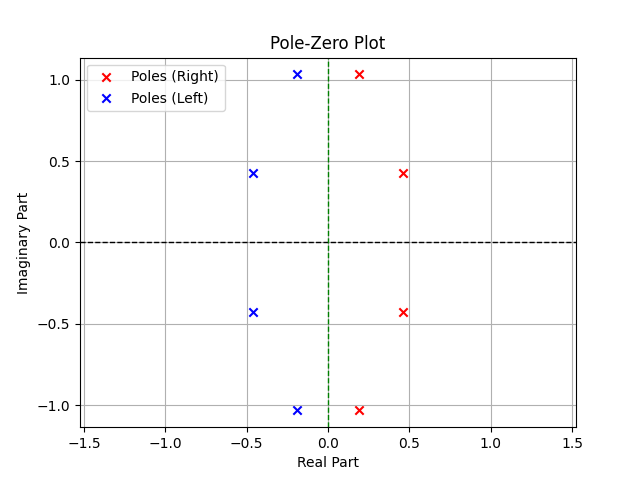
\includegraphics[width=1\columnwidth]{figs/Pole_Zero_plt.png}
\caption{The Pole zero plot and all the poles lie on an ellipse. The left and right poles have been identified as shown.}
\label{fig:pole_zero_plt}
\end{figure}
The poles in the left half of the plane are considered in the design as we intend to design a stable system.\\
Therefore the magnitude response is written as :- 
\begin{align}
    H_{a,LP}(s_L) &= \frac{G_{LP}}{\brak{s_L-s_5}\brak{s_L-s_6}\brak{s_L-s_7}\brak{s_L-s_8}}
\end{align}
where $G_{LP}$ is the gain of the Low pass filter. Refer to \tabref{tab:values poles sk} for $s_k$ values.\\

We know that from \eqref{eq:mag_freq_response}:-
\begin{align}
    \abs{ H_{a,LP}(s_L)} &= \frac{1}{\sqrt{1+\epsilon^2}} \text{at} \hspace{5pt} \Omega_{L}=1 \implies s_{L} = j \label{eq:Gain_eq_LP} 
\end{align}
Substituting respective values in \eqref{eq:Gain_eq_LP} we get $G_{LP}=0.3125$
\begin{align}
     H_{a,LP}(s_L) &= \frac{0.3125}{\brak{s_L-s_5}\brak{s_L-s_6}\brak{s_L-s_7}\brak{s_L-s_8}}\\
     &= \frac{0.3125}{s^4 + 1.1068s^3 + 1.61245s^2 + 0.91397s + 0.33656}\label{eq:design}
\end{align}
\begin{figure}[H]
\centering
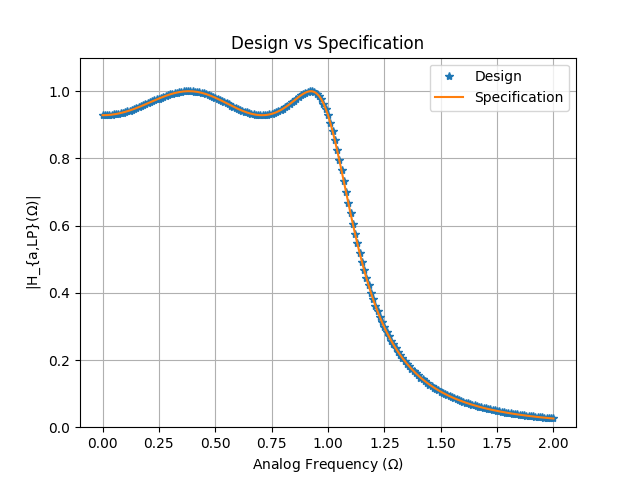
\includegraphics[width=1\columnwidth]{figs/Design_vs_Specification.png}
\caption{Design vs Specification corresponding to \eqref{eq:design} and \eqref{eq:specification}}
\label{fig:design_vs_specf}
\end{figure}

\item {The Band Pass Chebyschev Filter:} 
After verifying design with the required specifications the next step in design is to jump to required type of filter using frequency transformation. 
\begin{align}
    s_L &= \frac{s^2 + \Omega_0^2}{Bs} \\
    H_{a,BP}(s) &= G_{BP}H_{a,LP}(s_L)\vert_{s_L = \frac{s^2 + \Omega_0^2}{Bs}},
\end{align}
As there is one to one correspondence between the filters so $\Omega=\Omega_{p1}$ should correspond to $\Omega_{Lp}$
\begin{align}
    s &= j\Omega_{p1}\\
    s_{L} &= \frac{(j\Omega_{p1})^2 + \Omega_0^2}{B(j\Omega_{p1})} \label{eq:res1} \\ 
    \abs{H_{a,BP}(j\Omega_{p1})} &= 1 \\
    G_{BP}\abs{H_{a,LP}(s_L)} &= 1 \label{eq:res2}
\end{align}
Substituting \eqref{eq:res1} in \eqref{eq:res2} we obtain Gain of required bass pass filter:
\begin{align}
    G_{BP} &= 1.0771 
\end{align}
Thus the response in s domain 
\begin{align}
    H_{a,BP}\brak{s} &= \frac{9.8138\times 10^{-5}s^4}{s^8 + 0.108s^7 + 0.982s^6 + 0.079s^5 + 0.358s^4 + 0.0192s^3 + 0.0574s^2 + 0.0015s + 0.0034} \label{eq:magnitude_bandpass_sdom}
\end{align}
The expressions in the s-domain and gain factors are computed by writing a Python code. \\
In Figure 3, we plot $\vert H_{a,BP}(j\Omega)\vert$ as a function of $\Omega$ for both positve as
well as negative frequencies.  We find that the passband and stopband frequencies in the figure
match well with those obtained analytically through the bilinear transformation.
\begin{figure}[H]
\centering
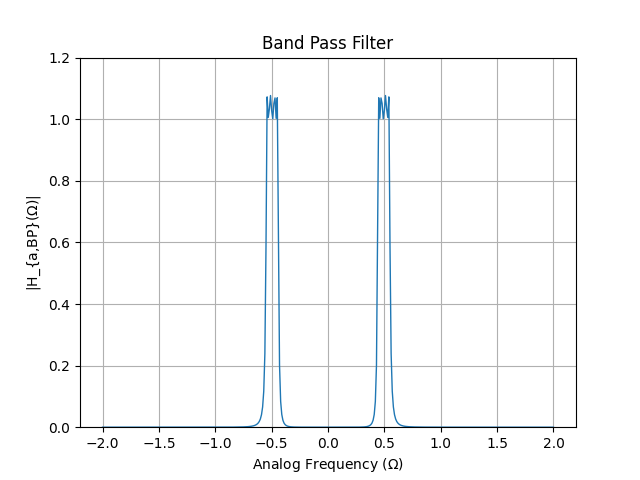
\includegraphics[width=1\columnwidth]{figs/Band_Pass_Filter.png}
\caption{The Analog Bandpass Magnitude Response from \eqref{eq:magnitude_bandpass_sdom}.The filter design specifications are satisfied}
\label{fig:band_pass_filter}
\end{figure}
\end{enumerate}

\subsection{The Digital Filter}
From the bilinear transformation, we obtain the digital bandpass filter from the corresponding analog filter as
\begin{align}
    H_{d,BP}(z) = GH_{a,BP}(s)\vert_{s = \frac{1-z^{-1}}{1 + z^{-1}}}
\end{align}
Substituting $s=\frac{1-z^{-1}}{1+z^{-1}}$ in \eqref{eq:magnitude_bandpass_sdom} and calculating expression using a python code we get :
\begin{align}
    H_{d,BP}(z) &= \frac{G\brak{z^{-8} - 4z^{-6} + 6z^{-4} - 4z^{-2} + 1.0}}{2.61 - 12.43z^{-1} + 32.16z^{-2} - 53.24z^{-3} + 61.99z^{-4} - 50.98z^{-5} + 29.48z^{-6} - 10.91z^{-7} + 2.19z^{-8}}
\end{align}

where $G=9.8138\times 10^{-5}$    
\begin{figure}[H]
\centering
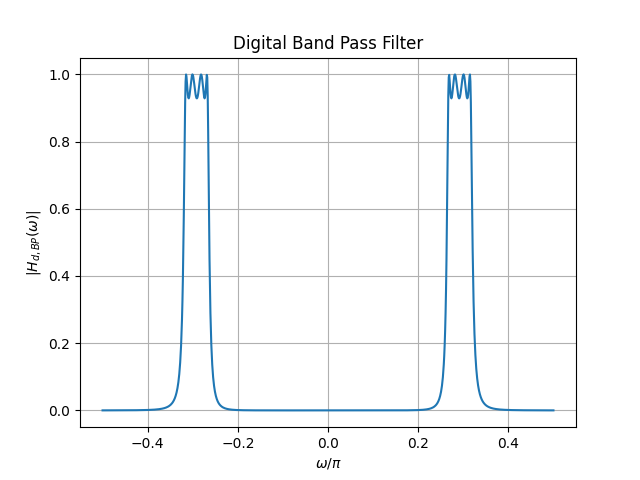
\includegraphics[width=1\columnwidth]{figs/Digital_BPF.png}
\caption{Digital Specifications are met. Passband and stopband frequencies are same}
\label{fig:Digital_BPF}
\end{figure}

\section{The FIR Filter}
We design the FIR filter by first obtaining the (non-causal) lowpass equivalent using the Kaiser window
and then
converting it to a causal bandpass filter.
\subsection{The Equivalent Lowpass Filter}
The lowpass filter has a passband frequency $\omega_l$ and transition band $\Delta \omega = 2\pi \frac{\Delta F}{F_s} = 0.0125\pi$.
The stopband tolerance is $\delta=0.15$.The cutoff-frequency is given by :
\begin{align}
    \omega_{l} &= \frac{\omega_{p1}-\omega_{p2}}{2}\\
                &= 0.025\pi
\end{align}
\begin{figure}[H]
\centering
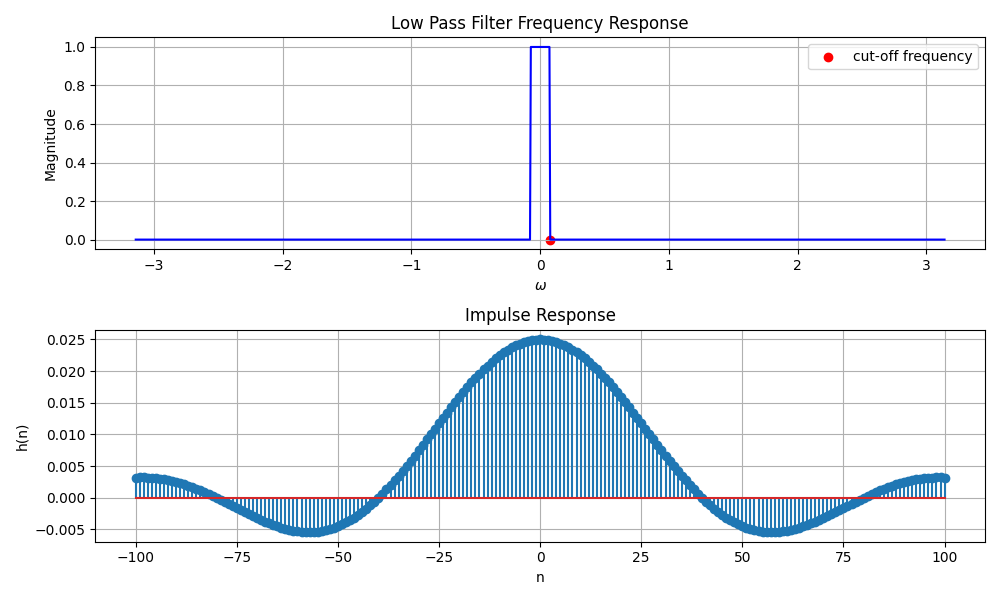
\includegraphics[width=1\columnwidth]{figs/LPF_FIR.png}
\caption{Frequency response and impulse response of an ideal Low Pass Filter}
\label{fig:LPF_FIR_1}
\end{figure}

The impulse response of ideal Low Pass Filter is given by :
\begin{align}
    h\brak{n} = 
\begin{cases} 
    \frac{w_l}{\pi}, & \text{if } n = 0 \\
    \frac{\sin(w_l n)}{n\pi}, & \text{if } n \neq 0
\end{cases} \label{eq:h(n)_for_LPF}
\end{align}
From \eqref{eq:h(n)_for_LPF} we conclude that $h\brak{n}$ for an ideal Low Pass Filter is not causal and can neither be made causal by introducing a finite delay. And $h\brak{n}$ do not converge and hence the system is unstable.
\subsection{The Kaiser Window}
Therefore we move on windowing the impulse response.A window function is chosen and multiplied. The Kaiser window is defined as
\begin{align}
    w(n) =
    \begin{cases}
    \frac{I_0\left[ \beta N \sqrt{1 - \left(\frac{n}{N}\right)^2} \right]}{I_0(\beta N)},
\indent -N \leq n \leq N, \indent \beta > 0 \nonumber \\
 0 \hspace{2.5 cm} \mbox{otherwise,}
 \end{cases}
\end{align}

\begin{enumerate}
\item  N is chosen according to
\begin{align}
    N \geq \frac{A-8}{4.57\Delta \omega},
\end{align}
where $A = -20\log_{10}\delta$.  Substituting the appropriate values from the design specifications, we obtain
$A = 16.4782$ and $N \geq 48$.


\item  $\beta$ is chosen according to

\begin{align}
    \beta N = \left\{ \begin{array}{ll} 0.1102(A-8.7) & A > 50 \\
0.5849(A-21)^{0.4}+ 0.07886(A-21) & 21 \leq A \leq 50 \\
0 & A < 21\end{array} \right.
\end{align}
The window function is defined as :
\begin{align}
    w\brak{n} = 
\begin{cases} 
    1, & \text{for } -48\leq n \leq 48 \\
    0, & \text{otherwise } 
\end{cases} \label{eq:w(n)_for_Kaiser}
\end{align}
Therefore the desired impulse response is :
\begin{align}
    h_{lp} &= h_{n}w_{n}
\end{align}
\begin{align}
    h\brak{n} = 
\begin{cases} 
    \frac{\sin(w_l n)}{n\pi},  & \text{for } -48\leq n \leq 48 \\
    0 &\text{otherwise}
\end{cases} \label{eq:h(n)-desired_for_LPF}
\end{align}
\end{enumerate}
\begin{figure}[H]
\centering
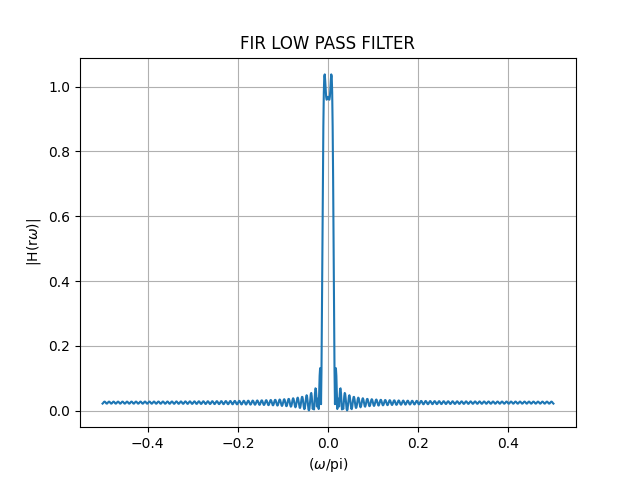
\includegraphics[width=1\columnwidth]{figs/FIR_Low_Filter.png}
\caption{Magnitude Response of Low Pass Filter after using Kaiser Window}
\label{fig:Kaiser_LPF_response}
\end{figure}

\subsection{The Equivalent Band Pass Filter}
A Band-Pass Filter (BPF) can be obtained by subtracting the magnitude response of a Low-Pass Filter (LPF) with cutoff frequency $\omega_{p1}$ from another LPF magnitude response with cutoff frequency $\omega_{p2}$.

\begin{align}
    h_{BP}\brak{n} = 
\begin{cases} 
    \frac{\sin(w_{p2} n)}{n\pi} -\frac{\sin\brak{\omega_{p1}n}}{n\pi},  & \text{for } n\neq 0\\\
    \frac{\omega_{p2}-\omega_{p1}}{\pi} &\text{for } n= 0
\end{cases} \label{eq:h(n)desired_for_LPF}
\end{align}
\begin{align}
     \frac{\sin(\omega_{p2} n)}{n\pi} -\frac{\sin\brak{\omega_{p1}n}}{n\pi} &= 2\cos{\brak{\frac{\omega_{p2}n+\omega_{p1}n}{2}}}\sin{\brak{\frac{\omega_{p2}n-\omega_{p1}n}{2}}}\\
            &= \frac{2\cos{\brak{0.292n\pi}}\sin{\brak{0.025n\pi}}}{n\pi}
\end{align}
Multipying by window function we get :
\begin{align}
    h_{BP}\brak{n} = 
\begin{cases} 
   \frac{2\cos{\brak{0.292n\pi}}\sin{\brak{0.025n\pi}}}{n\pi},  & \text{for } -48\leq n \leq 48 \\
    0 &\text{otherwise}
\end{cases} \label{eq:h_BP(n)desired_for_LPF}
\end{align}

\begin{figure}[H]
\centering
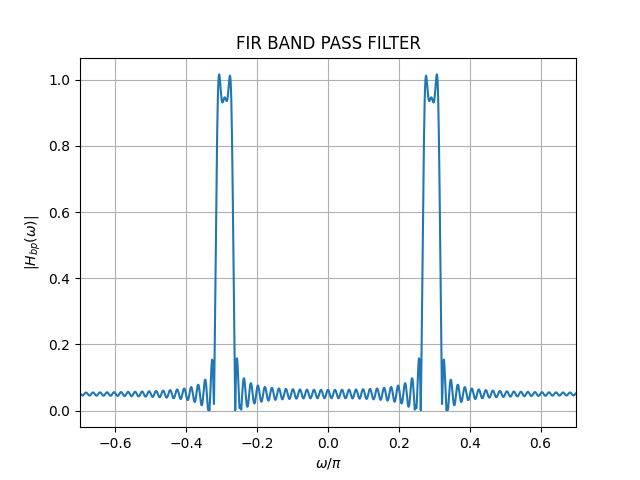
\includegraphics[width=1\columnwidth]{figs/FIR_Bandpass_Filter.png}
\caption{Magnitude Response of Band Pass Filter after using Kaiser Window}
\label{fig:Kaiser_BPF_response}
\end{figure}


\end{document}

